\begin{slide}{Beispiel: Graphenf�rbung (Aufgabe)}

\begin{minipage}{0.4\textwidth}
\includegraphics[width=7cm]{536970904.Dot.eps}
\end{minipage}%
\begin{minipage}{0.5\textwidth}
\begin{small}
\begin{verbatim}
Gesucht ist eine konfliktfreie 
Knoten-F�rbung des Graphen
Graph { knoten = mkSet [ 1 , 2 , 3 , 4 , 5 , 6 , 7 , 8 , 9 , 10 ]
  , kanten = mkSet [ kante 1 6 , kante 1 7 , kante 1 9 , kante 2 5
     , kante 2 7 , kante 2 8 , kante 2 9 , kante 3 6 , kante 3 7
     , kante 3 8 , kante 3 9 , kante 4 5 , kante 4 6 , kante 4 7
     , kante 5 6 , kante 5 10 , kante 6 7 , kante 6 8 , kante 6 10
     , kante 8 9 , kante 8 10 , kante 9 10 
     ] 
  }
mit h�chstens 3 verschiedenen Farben.
\end{verbatim}
\end{small}  
\end{minipage}

\end{slide}

\begin{slide}{Beispiel: Graphenf�rbung (L�sung)}
Eingabe:
\begin{small}
\begin{verbatim}
listToFM [ ( 1 , C ) , ( 2 , C ) , ( 3 , B ) , ( 4 , B ) , ( 5 , B )
    , ( 6 , A ) , ( 7 , A ) , ( 8 , C ) , ( 9 , C ) , ( 10 , C ) 
\end{verbatim}
\end{small}
Bewertung:
\begin{small}
\begin{verbatim}
Ist die Menge
    Knotenmenge des Graphen =
    mkSet [ 1 , 2 , 3 , 4 , 5 , 6 , 7 , 8 , 9 , 10 ]
Teilmenge der Menge
    gef�rbte Knoten = mkSet [ 1 , 2 , 3 , 4 , 5 , 6 , 7 , 8 , 9 , 10 ]
? Ja.
Diese Kante(n) verlaufen zwischen gleichfarbigen Knoten:
    [ kante 1 9 , kante 2 8 , kante 2 9 , kante 4 5 , kante 6 7
    , kante 8 9 , kante 8 10 , kante 9 10 ]
\end{verbatim}
\end{small}

\end{slide}

\begin{slide}{Typische Anwendung}

Problem (Bsp: 3SAT)
\begin{itemize}
\item Instanz: eine Formel in 3-KNF
\item L�sung: eine erf�llende Belegung
\end{itemize}

Ablauf mit \autotool\ :
\begin{itemize}
\item Tutor konfiguriert Generator
\item \autotool\ w�rfelt Instanz
  (f�r jeden Studenten eine andere)
\item Student gibt (vermutete) L�sung ein
\item \autotool\ verifiziert L�sung,
  gibt ausf�hrlichen Bericht (sofort)
\end{itemize}

\end{slide}




\begin{slide}{Beispiel: Graphenf�rbung (Konfiguration)}

das hat der Tutor eingestellt:
\begin{itemize}
\item Semantik:
Aufgabentyp: \verb|Col-Quiz| und Parameter
\begin{verbatim}
Config { nodes = 10 , edges = 30 , chi = 3 }
\end{verbatim}
\item Verwaltung:

Hochschule, Vorlesung, Aufgabe, Bearbeitungszeitraum, Wichtigkeit
\end{itemize}



\end{slide}
